\label{chapter:word2vec}


In this part I used assignment2 from cs224n, 2021 Stanford NLP course as my base code. Different Word2Vec models are trained for each label which exist in BBC data set. Headline is concatenated with body of each news for as input text for the model. Each models trains for 40000 iteration. It took about 5 hours for each label. Wights of models are saved is "models/word2vec" directory. Most 30 repeated words are chosen from each label. Images - , - , - and - shows distribution of each model on a 2D map. 


\section{Iran News}
After training word2vec model we exoect to see words with same meaning appear near to ech other and words with far meaning and context place far from others on each map.
\begin{figure}[h]
	\centering
	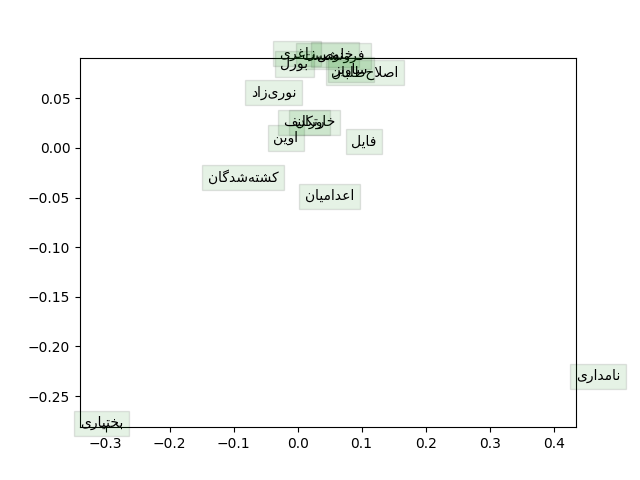
\includegraphics[width=10cm]{../reports/word2vec/word_vectors_ايران.png}
	\caption{Sub-words vocab example}
	\label{fig:word2veciran}
\end{figure}


\section{Art News}
\begin{figure}[h]
	\centering
	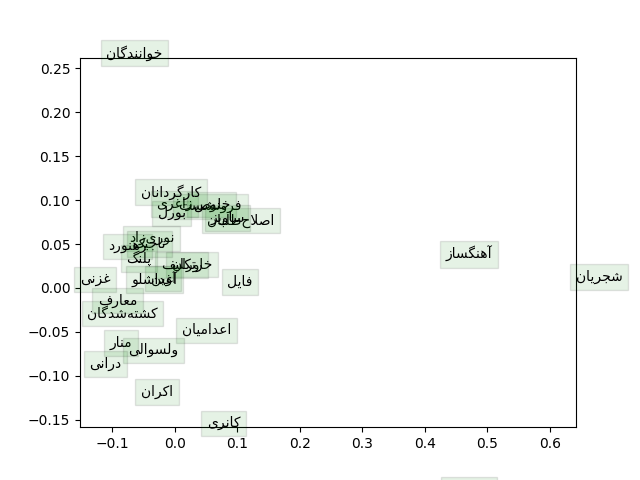
\includegraphics[width=10cm]{../reports/word2vec/word_vectors_هنر.png}
	\caption{Sub-words vocab example}
	\label{fig:word2vecart}
\end{figure}


\section{Sport News}
\begin{figure}[h]
	\centering
	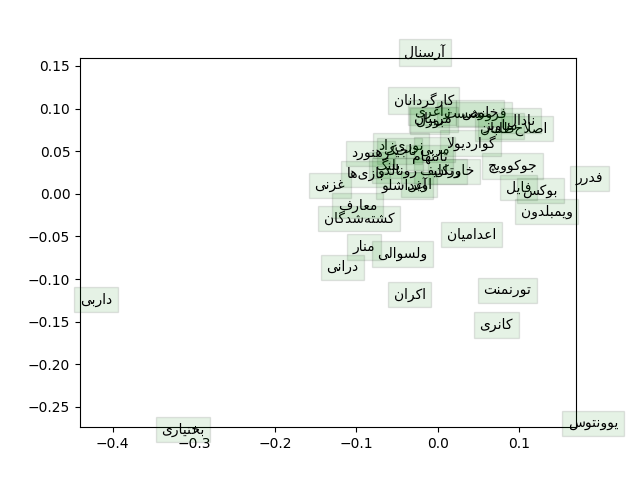
\includegraphics[width=10cm]{../reports/word2vec/word_vectors_ورزش.png}
	\caption{Sub-words vocab example}
	\label{fig:word2vecsport}
\end{figure}


\section{Economic News}
In map \ref{fig:word2vececon} words in car and it's factory are gathered in the left part of the image.
\begin{figure}[h]
	\centering
	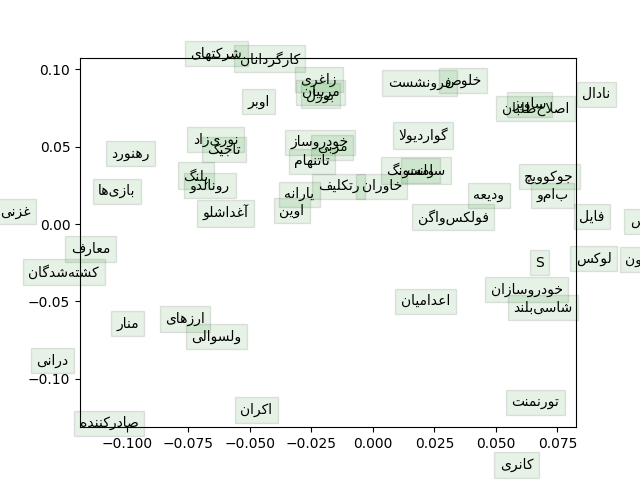
\includegraphics[width=10cm]{../reports/word2vec/word_vectors_اقتصاد.png}
	\caption{Sub-words vocab example}
	\label{fig:word2vececon}
\end{figure}

\section{Science News}
At map \ref{fig:word2vecsience} words are overlapped and it's not easy to distinguish them. Equivalent of two words Astronauts and UFO persia are in same context and located almost near to each other and far from others. Two other words are composer and name of a popular Iranian singer, Shajarian, are placed next to each other.
\begin{figure}[h]
	\centering
	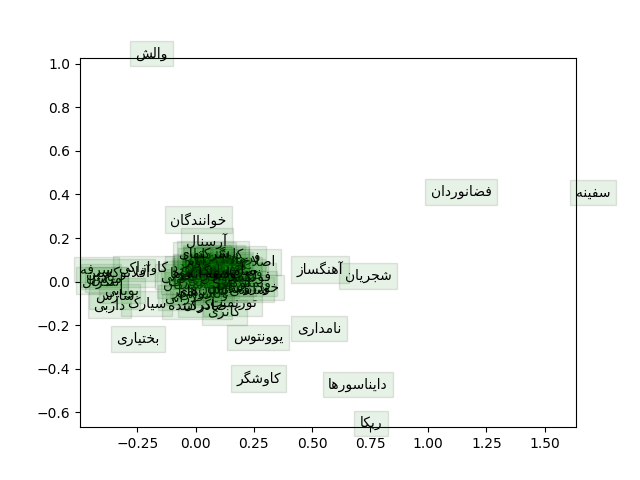
\includegraphics[width=10cm]{../reports/word2vec/word_vectors_دانش.png}
	\caption{Sub-words vocab example}
	\label{fig:word2vecsience}
\end{figure}
